% !TEX root = ../main.tex
% SECTION 1: ELEKTRISCHES FELD
% ============================================================

\StartChapter{Elektrisches Feld}

\begin{runintext}
Kräfte und Felder von Ladungen/Verteilungen: \ZSFkeyword*{Coulomb-Kraft}, \ZSFkeyword*{Dipole}, Feldlinien, Fluss, \ZSFkeyword*{Gauss-Gesetz}.
\end{runintext}

\SubsectionBar[sec:coulomb-charge]{Ladung, Coulomb}
\ZSFindex{Coulomb'sches Gesetz}
\ZSFindexsee{Gesetz von Coulomb}{Coulomb'sches Gesetz}
\ZSFindexsee{Coulomb-Kraft}{Coulomb'sches Gesetz}
\ZSFindex{Kraft / Kraft auf Leiter}
\ZSFindex{Elementarladung}
\ZSFindex{Zentripetalkraft}
\ZSFindex{Kreisbahn}
\begin{runintext}
Ladungserhaltung. \ZSFkeyword{Leiter} (freie Ladungen) vs. Nichtleiter. \ZSFkeyword{Erdung}: $\varphi=0$. \ZSFkeyword{Influenz}: erden $\to$ nähern $\to$ trennen $\to$ entfernen. \ZSFkeyword{Faraday-Käfig}: innen $E=0$. Kraft zwischen \ZSFkeyword[Punktladung]{Punktladungen} bei Abstand $r$.
\end{runintext}
\begin{defbox}[Elementarladung]
\ZSFkeyword[Ladung / Ladungsquantisierung]{Quantisierung}: Ladung in Vielfachen von $e$. Elektron: $-e$, Proton: $+e$.
\end{defbox}
\begin{formulabox}
\[ e = 1{,}60 \times 10^{-19}\,\si{C} \]
\formulanote{Zweck: Betrag der Elementarladung.}
\end{formulabox}
\begin{defbox}[Coulomb'sches Gesetz]
Kraft von $q_1$ auf $q_2$ im Abstand $r$; $\hat{r}$ von $q_1$ nach $q_2$.
\end{defbox}
\begin{formulabox}
\[ \begin{aligned}
\vec{F} &= \frac{1}{4\pi\varepsilon_0}\,\frac{q_1 q_2}{r^2}\,\hat{r} \\[-1pt]
m\,\frac{v^2}{r} &= \frac{1}{4\pi\varepsilon_0}\,\frac{|q_1 q_2|}{r^2} \quad \text{Kreisbahn ($F_{\mathrm{C}} = F_{\mathrm{Z}}$)}
\end{aligned} \]
\formulanote{Kraft zwischen Punktladungen \& Kreisbahn im E-Feld.}
\end{formulabox}

\SubsectionBar[sec:efield-superposition]{Elektrisches Feld, Superposition}
\ZSFindex{E-Feld / Elektrisches Feld}
\ZSFindex{Superposition}
\begin{runintext}
Formeln für das \ZSFkeyword*{elektrische Feld} $\vec{E}$ einer oder mehrerer Ladungen; $\vec{E}$ ist die Kraft $\vec{F}$ pro Probeladung $q_0$.
\end{runintext}
\begin{formulabox}
\[ \vec{E} = \frac{\vec{F}}{q_0} \qquad \vec{E} = \frac{1}{4\pi\varepsilon_0}\,\frac{q}{r^2}\,\hat{r} \quad \text{(Punktladung)} \]
\formulanote{Definition elektrisches Feld ($\vec{F}$ pro Probeladung $q_0$) und Feld einer Punktladung $q$ im Abstand $r$. Einheiten: $1\,\si{N/C} = 1\,\si{V/m}$.}
\end{formulabox}

\begin{formulabox}
\[ \vec{E} = \sum_i \vec{E}_i = \sum_i \frac{1}{4\pi\varepsilon_0}\,\frac{q_i}{r_i^2}\,\hat{r}_i \quad \text{Superposition} \]
\formulanote{\ZSFkeyword{Superposition}: Überlagerung der Felder mehrerer Punktladungen.}
\formulasep
\[ \vec{r} = \vec{r}_{\mathrm{Ziel}} - \vec{r}_{\mathrm{Quelle}} \quad \implies \quad \hat{r} = \frac{\vec{r}}{r} \]
\formulanote{Allgemeiner Richtungsvektor von Quelle (Ladung) zu Ziel (Feldpunkt).}
\formulasep
\[ \begin{aligned}
  \vec{r} &= (x-x_0)\vec{e}_x + (y-y_0)\vec{e}_y \\
  r &= \sqrt{(x-x_0)^2+(y-y_0)^2}
\end{aligned} \]
\formulanote{Kartesischer Abstand: Ziel/Feldpunkt $(x,y)$ vs. Quelle/Ladung $(x_0,y_0)$.}
\end{formulabox}

\ZSFindex{Spiegelladung}
\ZSFindex{Methode der Spiegelladungen}
\begin{runintext}
\ZSFkeyword{Feldlinien}: von $+$ nach $-$; lokale Dichte $\propto$ Feldstärke $|\vec{E}|$. \ZSFkeyword{Spiegelladung} (geerdete unendliche Leiterfläche): Spiegle die reale Ladungsverteilung an der Leiterfläche und kehre ihr Vorzeichen um; Feld im physikalischen Halbraum ($y>0$) durch Superposition. Bsp: $+\lambda \text{ bei } y=h \Rightarrow -\lambda \text{ bei } y=-h$.
\end{runintext}


\SubsectionBar[sec:dipole]{Dipol}
\ZSFindex{Kraft / Kraft auf Leiter}
\begin{runintext}
Formeln für \ZSFkeyword{Dipolmoment}, \ZSFkeyword{Drehmoment} und Energie eines Dipols im Feld; brauchst du bei Aufgaben zu polaren Molekülen oder kleinen Ladungspaaren im homogenen \ZSFkeyword*{elektrischen Feld}. \ZSFkeyword{Dipol}: zwei entgegengesetzt gleiche Ladungen, Abstand $\vec{\ell}$ (von $-$ nach $+$).
\end{runintext}

\begin{defbox}[Elektrischer Dipol \& Feldlinien]
\begin{splitbox}[0.65]
    \centering
    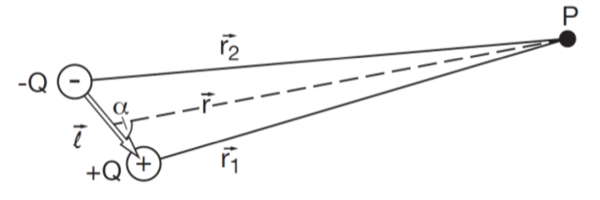
\includegraphics[width=\linewidth, keepaspectratio]{graphics/electric_dipole.png}
    \ZSFfigcaption{Zwei Ladungen $\pm q$ im Abstand $\vec{\ell}$}
    \tcblower
    \centering
    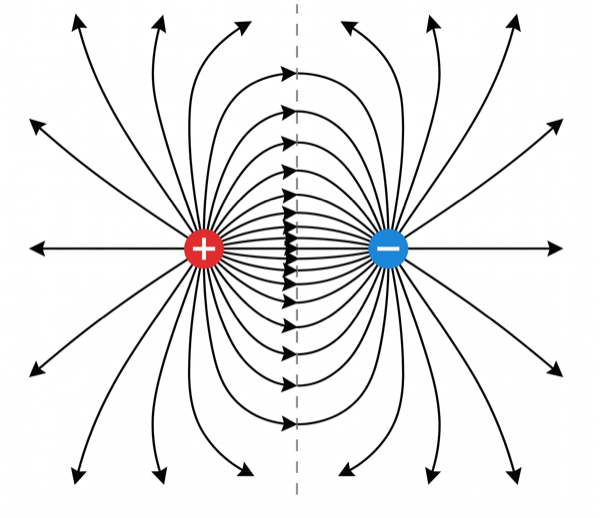
\includegraphics[width=\linewidth, keepaspectratio]{graphics/Elektrostatik_Dipol_Feldlinien_Symmetrie.png}
    \ZSFfigcaption{Feldlinien verlaufen von $+$ nach $-$}
\end{splitbox}
\end{defbox}

\begin{formulabox}
\[ \vec{p} = q\,\vec{\ell} \quad \text{Dipolmoment} \]
\formulanote{Zweck: Definition des elektrischen Dipolmoments.}
\formulasep
\[ \vec{M} = \vec{p} \times \vec{E} \quad \text{Drehmoment (homogenes E-Feld)} \]
\formulanote{Zweck: Drehmoment auf Dipol im elektrischen Feld.}
\formulasep
\[ E_{\mathrm{pot}} = -\vec{p}\cdot\vec{E} + U_0 \quad \text{($U_0$ oft $=0$)} \]
\formulanote{Zweck: Potenzielle Energie des Dipols im elektrischen Feld.}
\formulasep
\[ \vec{E}_{\mathrm{axial}} \approx \frac{1}{4\pi\varepsilon_0}\frac{2\vec{p}}{r^3}, \quad \vec{E}_{\mathrm{quer}} \approx -\frac{1}{4\pi\varepsilon_0}\frac{\vec{p}}{r^3} \quad (r \gg \ell) \]
\formulanote{Zweck: Dipol-Fernfeld auf Achse (axial) und quer dazu (Mittelsenkrechte).}
\end{formulabox}
\begin{runintext}
\ZSFkeyword*{Polare Moleküle}: permanentes $\vec{p}$; nichtpolar: induzierbar.
\end{runintext}

\SubsectionBar[sec:charge-distributions]{Ladungsverteilungen}
\ZSFindex{Flächenladungsdichte}
\ZSFindex{Linienladungsdichte}
\begin{runintext}
Formel zur Berechnung des \ZSFkeyword*{elektrischen Feldes} \ZSFkeyword[Ladungsverteilung]{kontinuierlicher Ladungsverteilungen} über ein Integral; bei ausgedehnten Ladungswolken, Drähten oder Flächen.
\end{runintext}
\begin{formulabox}
\[ \vec{E} = \int \mathrm{d}\vec{E} = \frac{1}{4\pi\varepsilon_0} \int \frac{\mathrm{d}q}{r^2}\,\hat{r} \]
\formulanote{Integration über Ladungselemente: $\mathrm{d}q = \rho\,\mathrm{d}V$ (Raum) / $\sigma\,\mathrm{d}A$ (Fläche) / $\lambda\,\mathrm{d}\ell$ (Linie).}
\end{formulabox}
{%
\tcbset{zsfstatementstyle/.append style={breakable=true}}%
\begin{procedure}[Rezept zur Herleitung des elektrischen Feldes]
  \ProcStep{Ladungselement aufstellen}{%
    \[ \mathrm{d}q = \lambda\,\mathrm{d}x \quad / \quad \sigma\,\mathrm{d}A \quad / \quad \rho\,\mathrm{d}V \]
  }
  \ProcStep{Symmetrien nutzen \& Komponenten zerlegen}{%
    Nur relevante Feldrichtung betrachten.
    \[ \mathrm{d}E_x = \mathrm{d}E \cos\theta = \frac{1}{4\pi\varepsilon_0}\,\frac{\mathrm{d}q}{r^2}\cos\theta \]
    \formulanote{Tipp: Drücke $r$, $x$ und $\cos\theta$ geometrisch aus (oft über Winkel $\vartheta$, siehe Winkelparametrisierung \ZSFref{sec:1-winkel}).}
  }
  \tcbbreak
  \ProcStep{Aufintegrieren}{%
    Grenzen bestimmen und integrieren.
    \[ E_x = \int \mathrm{d}E_x \]
  }
\end{procedure}%
}

\SubsectionBar[sec:1-winkel]{Winkelparametrisierung}
\ZSFindex{Winkelparametrisierung}
\begin{runintext}
\ZSFkeyword*{Winkelparametrisierung}: Bei geraden Quellen ($\lambda, I$) mit Lotabstand $h$ ersetzt der Sichtwinkel $\vartheta$ den Ort $x$: Der Kürzungstrick $\frac{\mathrm{d}x}{r^2} = \frac{1}{h}\mathrm{d}\vartheta$ vereinfacht das Integral.
\end{runintext}

\begin{figbox}[Geometrie der Winkelparametrisierung]
\centering
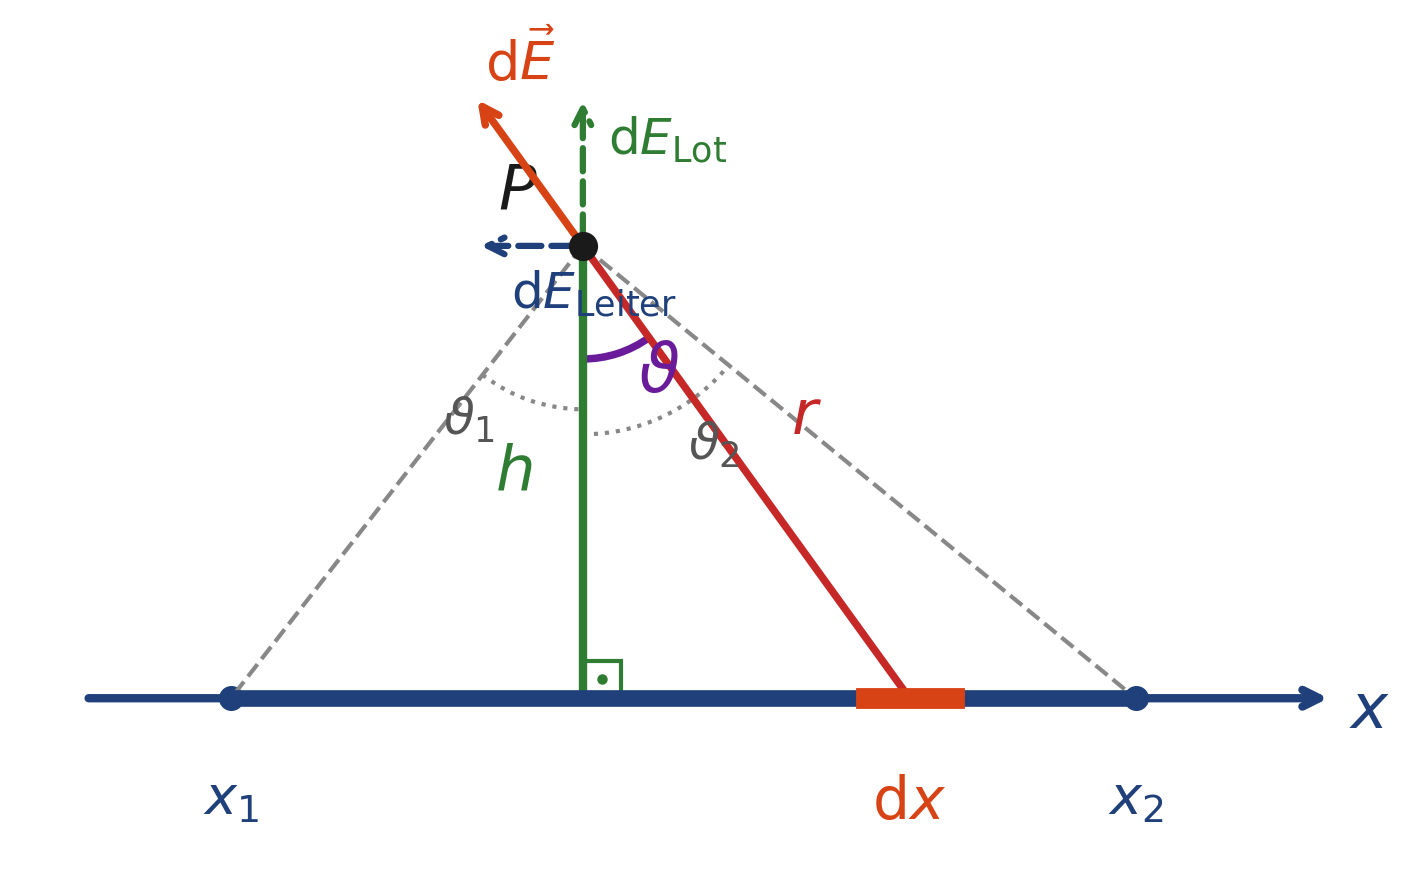
\includegraphics[width=\linewidth]{graphics/Winkelparametrisierung_Geometrie.png}
\ZSFfigcaption{Beobachtungspunkt $P$ im Lotabstand $h$. Sichtwinkel $\vartheta$ ersetzt Ortskoordinate $x$.}
\end{figbox}


\begin{formulabox}
\[
\begin{aligned}
  x &= h\tan\vartheta, & \mathrm{d}x &= \frac{h}{\cos^2\vartheta}\,\mathrm{d}\vartheta \\
  r &= \frac{h}{\cos\vartheta}, & \frac{\mathrm{d}x}{r^2} &= \frac{1}{h}\,\mathrm{d}\vartheta \quad \text{(\ZSFkeyword*{Kürzungstrick})}
\end{aligned}
\]
\formulanote{Der Abstand $r^2$ kürzt sich mit $\mathrm{d}x$ weg — übrig bleibt der Lotabstand $h$.}
\end{formulabox}

\begin{formulabox}
\[
\begin{aligned}
  E_{\mathrm{Lot}} &= \frac{\lambda}{4\pi\varepsilon_0 h}\Bigl[\sin\vartheta\Bigr]_{\vartheta_1}^{\vartheta_2} \\
  E_{\mathrm{Leiter}} &= \frac{\lambda}{4\pi\varepsilon_0 h}\Bigl[-\cos\vartheta\Bigr]_{\vartheta_1}^{\vartheta_2} \\
  B &= \frac{\mu_0 I}{4\pi h}\Bigl[\sin\vartheta\Bigr]_{\vartheta_1}^{\vartheta_2} \quad \text{(Biot-Savart)}
\end{aligned}
\]
\formulanote{Projektionen: $\cos\vartheta \to$ Lotkomponente ($E_{\mathrm{Lot}}, B$), $\sin\vartheta \to$ Leiterrichtung ($E_{\mathrm{Leiter}}$).}
\end{formulabox}

\SubsectionBar[sec:electric-flux]{Elektrischer Fluss}
\begin{runintext}
Formel für den \ZSFkeyword[Elektrischer Fluss]{elektrischen Fluss} durch eine Fläche; brauchst du bei Feldlinienanzahl/Fluss durch eine Fläche und als Vorbereitung für das \ZSFkeyword*{Gauss-Gesetz}.
\end{runintext}
\begin{formulabox}
\[ \Phi_{\mathrm{el}} = \lim_{\Delta A_i\to 0} \sum_i \vec{E}_i\cdot\Delta\vec{A}_i = \int_A \vec{E}\cdot\mathrm{d}\vec{A} \]
\formulanote{Zweck: Elektrischer Fluss durch Fläche $A$ (anschaulich: Nettozahl der Feldlinien durch $A$).}
\end{formulabox}

\columnbreak
\SubsectionBar[sec:gauss-law]{Gauss}
\ZSFindex{Gauss-Gesetz / Gesetz von Gauss}
\ZSFindex{Gauss-Fläche}
\ZSFindex{Flächenladungsdichte}
\begin{runintext}
Integralform des \ZSFkeyword*[Gauss'sches Gesetz]{Gauss-Gesetzes} und Randwerte am Leiter; nützlich zur Bestimmung von \ZSFkeyword*{elektrischen Feldern} stark symmetrischer Ladungsverteilungen ohne explizite Integration.
\end{runintext}
\begin{formulabox}
\[ \Phi_{\mathrm{el}} = \oint_A \vec{E}\cdot\mathrm{d}\vec{A} = \oint_A E_n\,\mathrm{d}A = \frac{q_{\mathrm{innen}}}{\varepsilon_0} \]
\formulanote{Zweck: Gauss'sches Gesetz; Fluss $\propto$ eingeschlossene Ladung.}
\end{formulabox}

\begin{figbox}[Visualisierung Gauss'sches Gesetz]
\centering
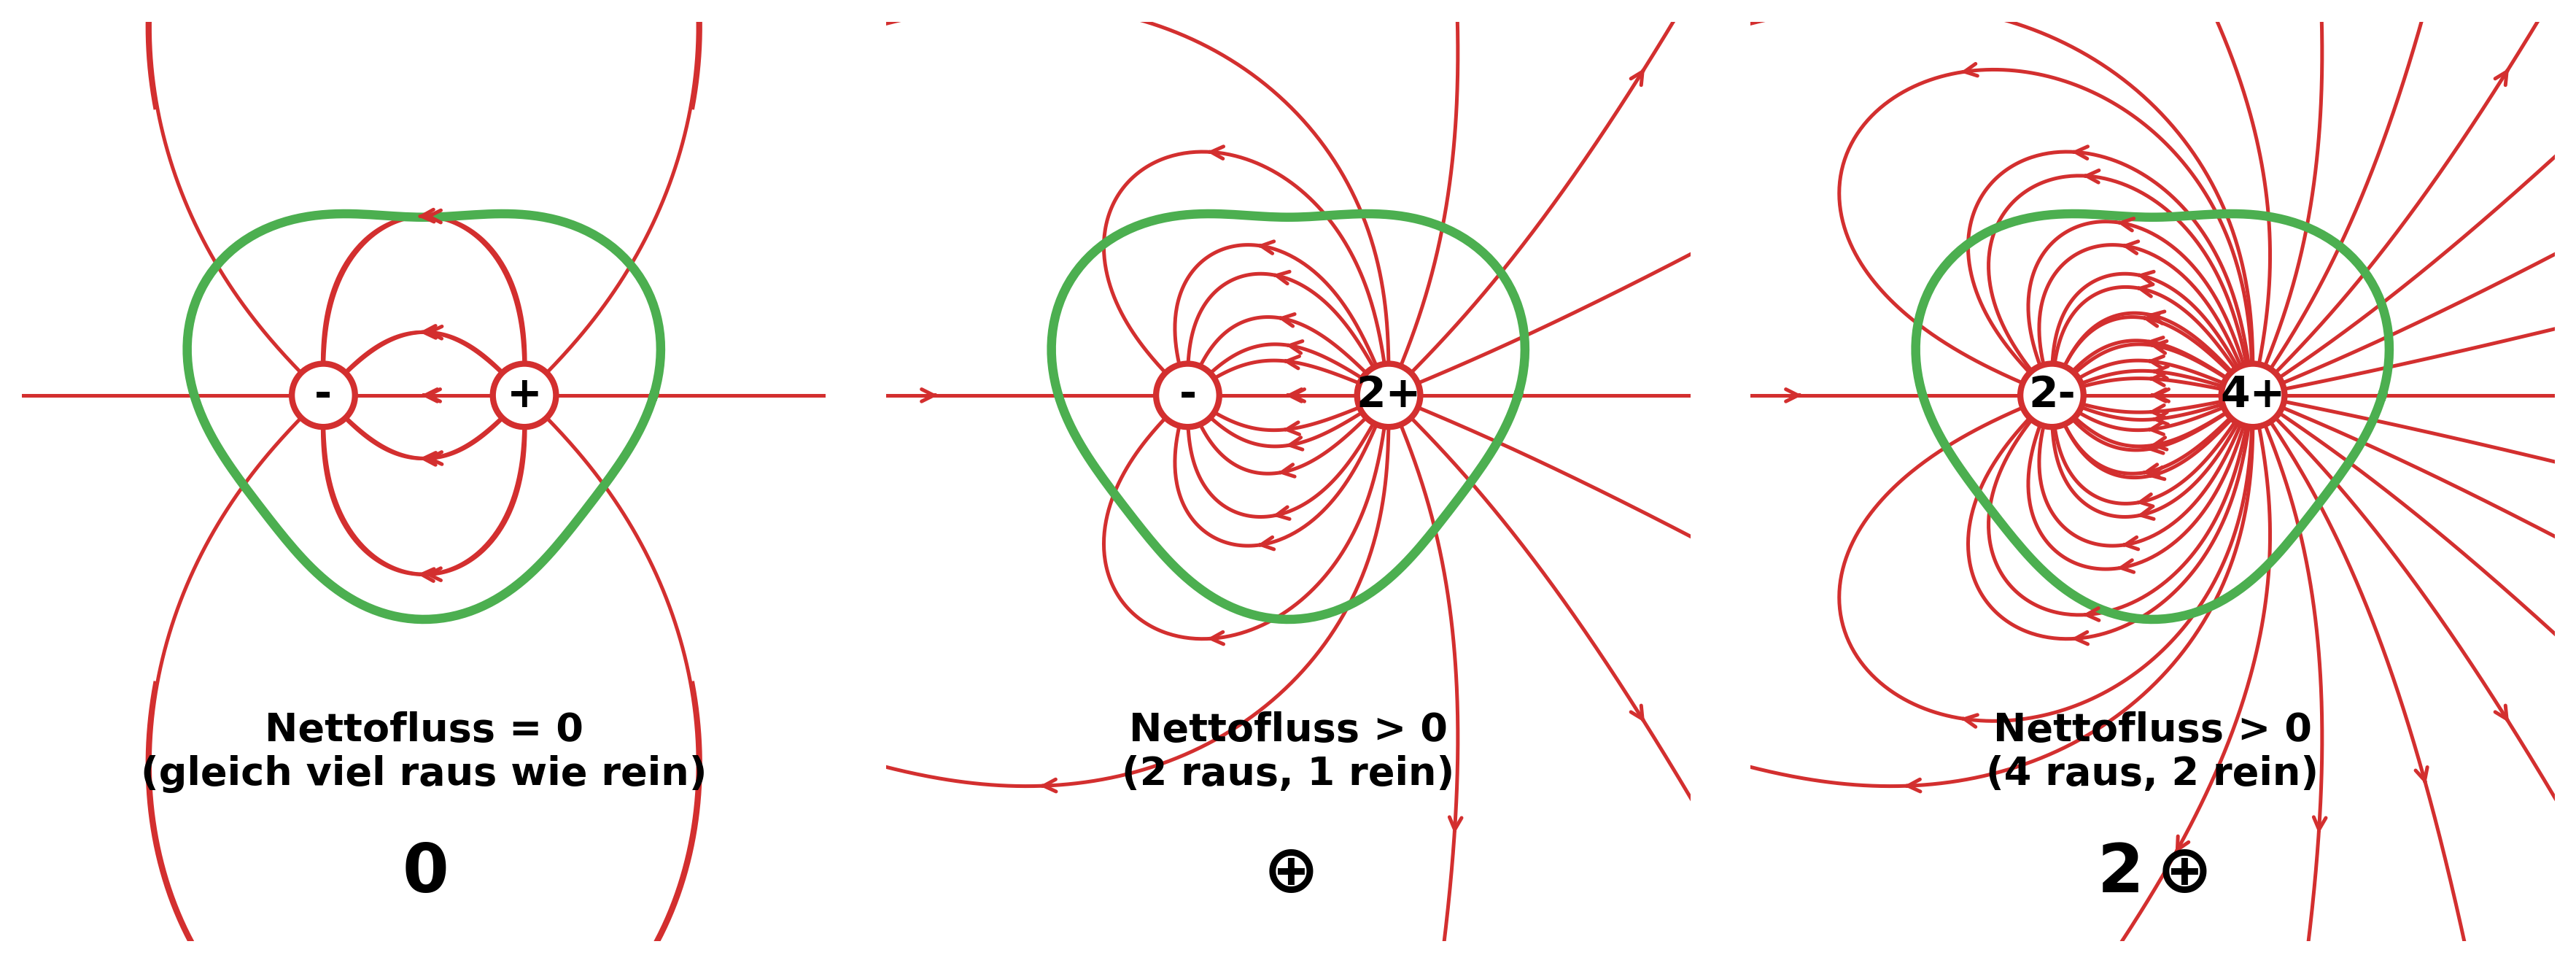
\includegraphics[width=\linewidth, keepaspectratio]{graphics/gauss_flux_explanation.png}
\ZSFfigcaption{Netto-Fluss $\Phi_{\mathrm{el}}$ (austretende Feldlinien) hängt nur von eingeschlossener Netto-Ladung ab.}
\end{figbox}
\ZSFgapS

\begin{formulabox}
\[
\begin{gathered}
\oint_A \vec{E}\cdot\mathrm{d}\vec{A} = E(r)\,4\pi r^2 = \frac{q_{\mathrm{innen}}(r)}{\varepsilon_0} \\[-2pt]
\text{Kugelsymmetrie (auf Kugelfläche ist $E$ konstant)}
\end{gathered}
\]
\[ E(r) = \frac{1}{4\pi\varepsilon_0}\,\frac{q_{\mathrm{innen}}(r)}{r^2} \]
\formulanote{Zweck: Vereinfachte Gauss-Form bei Kugelsymmetrie; kein neues Gesetz.}
\end{formulabox}
\begin{runintext}
\ZSFkeyword{Leiter}: Gesamte Ladung sitzt auf der Oberfläche; im Inneren gilt $E=0$ und $q=0$ (Spiegelladung: \ZSFref{sec:efield-superposition}).
\end{runintext}
\begin{formulabox}
\[ \Delta E_n = E_{n,+} - E_{n,-} = \frac{\sigma}{\varepsilon_0} \quad \text{Unstetigkeit} \]
\[ E_n = \frac{\sigma}{\varepsilon_0} \quad \text{unmittelbar ausserhalb Leiter} \]
\formulanote{Zweck: Feld-Sprung ($\Delta E_n$) beim Durchqueren einer geladenen Fläche. Am Leiter gilt $E_{n,-}=0$ (innen) $\implies E_n = \frac{\sigma}{\varepsilon_0}$ (aussen).}
\end{formulabox}

\SubsectionBar[sec:spherical-fields]{Kugelsymmetrische Ladungsverteilungen}
\ZSFindex{Kugelschale}
\ZSFindex{Vollkugel}
\ZSFindex{Dicke Kugelschale}
\begin{runintext}
Bei Kugelsymmetrie hängt das Feld nur vom Radius $r$ ab. Mit dem Gauss-Gesetz wird deshalb in jedem Bereich nur $q_{\mathrm{innen}}(r)$ bestimmt.
\end{runintext}

\begin{formulabox}
\[
\begin{aligned}
\text{Dünne Kugelschale:}\quad &E(r)=0 &&(r<R),\\
&E(r)=\frac{1}{4\pi\varepsilon_0}\frac{Q}{r^2} &&(r>R),\\[1ex]
\text{homogene Vollkugel:}\quad &\vec E(r)=\frac{\rho}{3\varepsilon_0}\,\vec r &&(r<R),\\
&E(r)=\frac{1}{4\pi\varepsilon_0}\frac{Q}{r^2} &&(r>R).
\end{aligned}
\]
\formulanote{Innen ist bei der dünnen Schale keine Ladung eingeschlossen; bei der Vollkugel wächst $q_{\mathrm{innen}}(r)$ mit dem Volumen.}
\end{formulabox}

\begin{formulabox}[Dicke Kugelschale]
\[
\begin{aligned}
q_{\mathrm{innen}}(r)&=\frac{4\pi\rho}{3}\left(r^3-R_i^3\right)
&& (R_i<r<R_a),
\end{aligned}
\]
\[
E(r)=\begin{cases}
0, & r<R_i,\\[1ex]
\dfrac{\rho}{3\varepsilon_0}\left(r-\dfrac{R_i^3}{r^2}\right), & R_i<r<R_a,\\[2ex]
\dfrac{1}{4\pi\varepsilon_0}\dfrac{Q}{r^2}, & r>R_a.
\end{cases}
\]
\formulanote{Im Material zählt nur die Kugelschale zwischen $R_i$ und dem betrachteten Radius $r$; ausserhalb ist die Gesamtladung $Q$ eingeschlossen.}
\end{formulabox}

\ZSFgapS
\begin{procedure}[Ortsabhängige Ladungsdichte $\rho(r)$]
  \ProcStep{Eingeschlossene Ladung für $r<R$}{%
    \ZSFdanger{Achtung:} Falls $\rho = \rho(r)$, zuerst die eingeschlossene Ladung bis zum aktuellen Radius bestimmen.
    \[ q_{\mathrm{in}}(r) = 4\pi \int_0^r \rho(r') (r')^2\,\mathrm{d}r' \]
  }
  \ProcStep{Elektrisches Feld innen bestimmen}{%
    \[ E_{\mathrm{innen}}(r) = \frac{q_{\mathrm{in}}(r)}{4\pi\varepsilon_0 r^2} = \frac{1}{\varepsilon_0 r^2}\int_0^r \rho(r') (r')^2\,\mathrm{d}r' \]
    \formulanote{Aussen ($r > R$): Das Feld verhält sich wie eine Punktladung \ZSFref{sec:efield-superposition} mit der Gesamtladung $Q = q_{\mathrm{in}}(R)$ im Ursprung.}
  }
\end{procedure}

\SubsectionBar[sec:standard-fields]{Standardgeometrien ausserhalb der Kugelsymmetrie}
\ZSFindex{Linienladungsdichte}
\begin{runintext}
Fertige Resultate für typische nicht-kugelsymmetrische Verteilungen; praktisch zum schnellen Einsetzen in Zahlenaufgaben mit Linienladung, Ring, Scheibe und Ebene.
\end{runintext}
\begin{formulabox}
\[ \vec{E} = \frac{1}{2\pi\varepsilon_0}\,\frac{\lambda}{r_\perp}\,\hat{r}_\perp \]
\formulanote{Gerader, sehr langer geladener Draht; $r_\perp$ Lotabstand.}
\end{formulabox}

\begin{formulabox}
\[ \lambda = \sigma\,2\pi r \quad \text{zylindrischer Leiter} \]
\formulanote{Zweck: Umrechnung zwischen Flächenladungsdichte $\sigma$ und Linienladungsdichte $\lambda$ bei Radius $r$.}
\end{formulabox}

\begin{formulabox}
\[ E_z = \frac{1}{4\pi\varepsilon_0}\,\frac{qz}{(z^2+a^2)^{3/2}} \]
\formulanote{Ring (Radius $a$), Feldpunkt auf der Achse durch die Ringmitte.}
\end{formulabox}

\begin{formulabox}
\[ E_z = \frac{\sigma}{2\varepsilon_0}\,\sgn(z)\left(1 - \left(1+\frac{r_S^2}{z^2}\right)^{-1/2}\right) \]
\formulanote{Flache runde Platte (Radius $r_S$), Feldpunkt auf ihrer Achse.}
\end{formulabox}

\begin{formulabox}
\[ E = E_z = \sgn(z)\,\frac{\sigma}{2\varepsilon_0} \]
\formulanote{Unendliche Ebene: sehr grosse, gleichmässig geladene Fläche; $z$ Abstand davon. $\sgn(z) = \pm 1$ (Vorzeichen von $z$): Feld kehrt beim Durchtritt die Richtung um. \ZSFdanger{Faktor 2:} an der Leiteroberfläche gilt $\sigma/\varepsilon_0$ \ZSFref{sec:gauss-law}, weil innen $E = 0$ ist und das ganze Feld nach aussen geht.}
\end{formulabox}

% ============================================================
